\documentclass{article}
\usepackage{amsmath}
\usepackage{tikz}
\usepackage{pgfplots}

\begin{document}
    Naj bo \(U(x,y) = U_{x,y}\) matrika
    \begin{align*}
        \Delta u(x,y) = U_{xx} + U_{yy}\\
        h\cdot U_x = U(x) - U(x+1)\\
        h^2\cdot U_{xx} = U(x-1, y) - 2U(x,y) + U(x+1,y)\\
        h^2\cdot U_{yy} = U(x, y-1) - 2U(x,y) + U(x, y+1)
    \end{align*}
    Če to damo skupaj, dobimo
    \begin{align*}
        \Delta U(x,y) + k(x,y)U(x,y) = 1\
        h^2 = U(x-1,y)+U(x+1,y)+U(x,y-1)+U(x,y+1) + (h^2\cdot k(x,y)- 4) U(x,y)
    \end{align*}
    Vemo, da je \(U(i,j)=0\) na \(\partial [-1,1]^2\) oziroma \(\{0,n\}\times [0,n]\) in obratno.
    \section{Naloga 4}

    Iters
    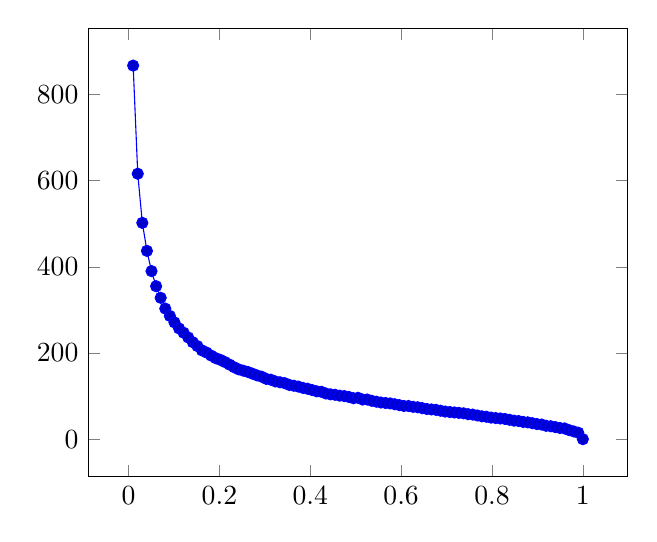
\begin{tikzpicture}
        \begin{axis}
        \addplot coordinates {
                (0.010101, 867)
                (0.020202, 616)
                (0.030303, 502)
                (0.040404, 437)
                (0.050505, 390)
                (0.0606061, 355)
                (0.0707071, 328)
                (0.0808081, 303)
                (0.0909091, 286)
                (0.10101, 271)
                (0.111111, 257)
                (0.121212, 247)
                (0.131313, 236)
                (0.141414, 225)
                (0.151515, 216)
                (0.161616, 206)
                (0.171717, 201)
                (0.181818, 194)
                (0.191919, 188)
                (0.20202, 184)
                (0.212121, 179)
                (0.222222, 173)
                (0.232323, 167)
                (0.242424, 162)
                (0.252525, 159)
                (0.262626, 156)
                (0.272727, 152)
                (0.282828, 148)
                (0.292929, 145)
                (0.30303, 140)
                (0.313131, 138)
                (0.323232, 134)
                (0.333333, 132)
                (0.343434, 130)
                (0.353535, 126)
                (0.363636, 124)
                (0.373737, 122)
                (0.383838, 119)
                (0.393939, 117)
                (0.40404, 114)
                (0.414141, 111)
                (0.424242, 110)
                (0.434343, 106)
                (0.444444, 104)
                (0.454545, 103)
                (0.464646, 101)
                (0.474747, 100)
                (0.484848, 98)
                (0.494949, 95)
                (0.50505, 96)
                (0.515152, 92)
                (0.525253, 92)
                (0.535354, 89)
                (0.545455, 87)
                (0.555556, 85)
                (0.565657, 84)
                (0.575758, 83)
                (0.585859, 81)
                (0.59596, 79)
                (0.606061, 77)
                (0.616162, 77)
                (0.626263, 75)
                (0.636364, 74)
                (0.646465, 72)
                (0.656566, 70)
                (0.666667, 69)
                (0.676768, 68)
                (0.686869, 66)
                (0.69697, 64)
                (0.707071, 63)
                (0.717172, 62)
                (0.727273, 61)
                (0.737374, 60)
                (0.747475, 58)
                (0.757576, 57)
                (0.767677, 55)
                (0.777778, 53)
                (0.787879, 52)
                (0.79798, 50)
                (0.808081, 49)
                (0.818182, 48)
                (0.828283, 47)
                (0.838384, 45)
                (0.848485, 43)
                (0.858586, 42)
                (0.868687, 40)
                (0.878788, 39)
                (0.888889, 37)
                (0.89899, 35)
                (0.909091, 34)
                (0.919192, 31)
                (0.929293, 30)
                (0.939394, 28)
                (0.949495, 26)
                (0.959596, 25)
                (0.969697, 21)
                (0.979798, 18)
                (0.989899, 15)
                (1, 0)
            };
        \end{axis}
    \end{tikzpicture}

    Alphas
    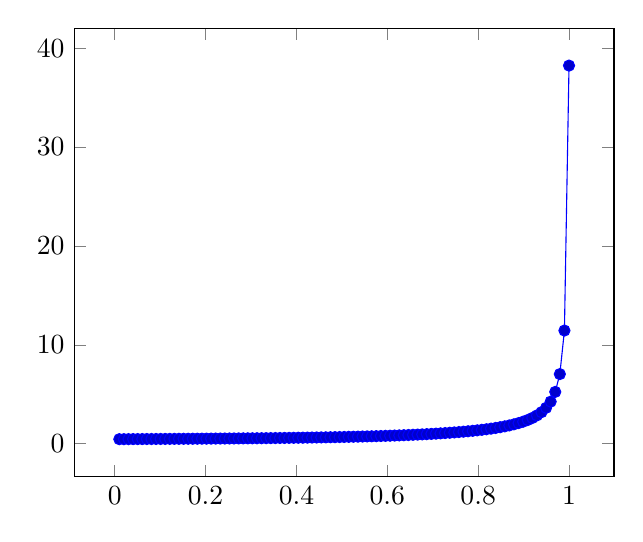
\begin{tikzpicture}
        \begin{axis}
        \addplot coordinates {
            (0.010101, 0.458222)
(0.020202, 0.460376)
(0.030303, 0.462818)
(0.040404, 0.465419)
(0.050505, 0.468106)
(0.0606061, 0.470839)
(0.0707071, 0.473596)
(0.0808081, 0.476368)
(0.0909091, 0.479151)
(0.10101, 0.481945)
(0.111111, 0.484754)
(0.121212, 0.487581)
(0.131313, 0.490431)
(0.141414, 0.493311)
(0.151515, 0.496226)
(0.161616, 0.499183)
(0.171717, 0.502188)
(0.181818, 0.505247)
(0.191919, 0.508369)
(0.20202, 0.511559)
(0.212121, 0.514824)
(0.222222, 0.518173)
(0.232323, 0.521612)
(0.242424, 0.525148)
(0.252525, 0.528789)
(0.262626, 0.532544)
(0.272727, 0.536419)
(0.282828, 0.540424)
(0.292929, 0.544566)
(0.30303, 0.548854)
(0.313131, 0.553297)
(0.323232, 0.557905)
(0.333333, 0.562688)
(0.343434, 0.567654)
(0.353535, 0.572815)
(0.363636, 0.578181)
(0.373737, 0.583763)
(0.383838, 0.589574)
(0.393939, 0.595625)
(0.40404, 0.601929)
(0.414141, 0.6085)
(0.424242, 0.615351)
(0.434343, 0.622498)
(0.444444, 0.629956)
(0.454545, 0.637741)
(0.464646, 0.645871)
(0.474747, 0.654363)
(0.484848, 0.663238)
(0.494949, 0.672515)
(0.50505, 0.682216)
(0.515152, 0.692364)
(0.525253, 0.702984)
(0.535354, 0.714102)
(0.545455, 0.725746)
(0.555556, 0.737945)
(0.565657, 0.750733)
(0.575758, 0.764144)
(0.585859, 0.778214)
(0.59596, 0.792984)
(0.606061, 0.808499)
(0.616162, 0.824805)
(0.626263, 0.841953)
(0.636364, 0.860001)
(0.646465, 0.879011)
(0.656566, 0.899049)
(0.666667, 0.920191)
(0.676768, 0.942519)
(0.686869, 0.966126)
(0.69697, 0.991113)
(0.707071, 1.0176)
(0.717172, 1.0457)
(0.727273, 1.07558)
(0.737374, 1.10739)
(0.747475, 1.14132)
(0.757576, 1.17759)
(0.767677, 1.21645)
(0.777778, 1.25818)
(0.787879, 1.30314)
(0.79798, 1.35172)
(0.808081, 1.40439)
(0.818182, 1.46175)
(0.828283, 1.52448)
(0.838384, 1.59345)
(0.848485, 1.66974)
(0.858586, 1.75473)
(0.868687, 1.85016)
(0.878788, 1.95836)
(0.888889, 2.08245)
(0.89899, 2.22673)
(0.909091, 2.39733)
(0.919192, 2.60328)
(0.929293, 2.85855)
(0.939394, 3.18593)
(0.949495, 3.6253)
(0.959596, 4.25349)
(0.969697, 5.23951)
(0.979798, 7.04002)
(0.989899, 11.4415)
(1, 38.2373)
            };
        \end{axis}
    \end{tikzpicture}

\end{document}